% Emacs settings: -*-mode: latex; TeX-master: "manual.tex"; -*-

\chapter{Source components}
\label{c:source}
\index{Sources|textbf}
\index{Library!Components!sources}

\MCS\ contains a number of different source components,
and any simulation will usually contain exactly one of these sources.
The main function of a source is to determine a set of initial
parameters $({\bf r}, {\bf v}, t)$
for each neutron ray. This is done by Monte Carlo choices from
suitable distributions. For example, in most present sources
the initial position is
found from a uniform distribution over the source surface,
which can be chosen to be either circular or rectangular.
The initial neutron velocity is selected within an interval
of either the corresponding energy or the corresponding wavelength.
Polarization is not relevant for sources,
and we initialize the neutron average spin to zero: ${\bf s}=(0,0,0)$.

For time-of-flight sources, the choice of the emission time, $t$,
is being made on basis of detailed analytical expressions.
For other sources, $t$ is set to zero.
In the case one would like to use a steady state source
with time-of-flight settings,
the emission time of each neutron ray should be determined using
a Monte Carlo choice. This may be achieved by
the \verb+EXTEND+ keyword in the instrument description source
as in the example below:\index{Keyword!EXTEND}

\begin{verbatim}
  TRACE

  COMPONENT MySource=Source_gen(...) AT (...)
  EXTEND
  %{
    t = 1e-3*randpm1(); /* set time to +/- 1 ms */
  %}
\end{verbatim}

\subsection{Photon flux and Brilliance}
\label{s:xray-flux}
The flux of the sources deserves special attention. The total
intensity is defined as the sum of weights of all emitted xrays
during one simulation
(the unit of total photon weight is thus xrays per second).
The flux, $\psi$, at an instrument is defined as intensity per area perpendicular
to the beam direction.

The source flux, $\Phi$, is defined in different units:
the number of photon rays emitted per second from a
1~cm$^2$ area on the source surface,
with direction within a 1~ster.\ solid angle,
and with wavelength within a 1 {\AA} interval.
The total intensity of real neutrons emitted towards a given diaphragm
(units: n/sec) is therefore (for constant $\Phi$):
\begin{equation}
I_{\rm total} = \Phi A \Delta\Omega \Delta\lambda ,
\end{equation}
where $A$ is the source area, $\Delta\Omega$ is the solid angle of the
diaphragm as seen from the source surface, and $\Delta\lambda$ is the
width of the wavelength interval in which neutrons are emitted (assuming
a uniform wavelength spectrum).

The simulations are performed so that detector intensities
are independent of the number of neutron histories simulated
(although more neutron histories will give better statistics).
If $N_{\rm sim}$ denotes the number of
xray histories to simulate, the initial photon weight $p_0$ must be set to
\begin{equation}
\label{proprule}
p_0 = \frac{N_{\rm total}}{N_{\rm sim}} =
    \frac{\Phi(\lambda)}{N_{\rm sim}} A \Omega \Delta\lambda ,
\end{equation}
where the source flux is now given a $\lambda$-dependence.

As a start, we recommend new \MCS\ users to use the
{\bf Source\_simple} component.
Slightly more realistic sources are {\bf Source\_Maxwell\_3} for
continuous sources or {\bf Moderator} for time-of-flight sources.

Optimizers can dramatically improve the statistics, but may occasionally
give wrong results, due to misleaded optimization.
You should always check such simulations with (shorter) non-optimized ones.

Other ways to speed-up simulations are to read events from a file.
See section \ref{sources-seealso} for details.

\begin{figure}
  \begin{center}
    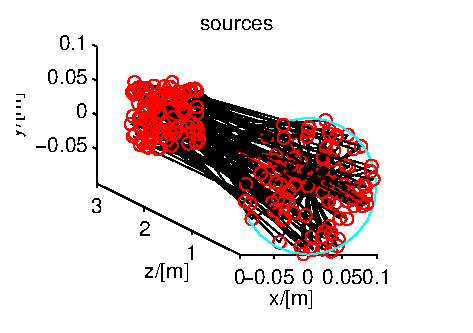
\includegraphics[width=0.75\textwidth]{figures/sources.eps}
  \end{center}
\caption{A circular source component (at z=0) emitting photon rays randomly, either from a model, or from a data file.}
\label{f:source}
\end{figure}

\newpage
\section{Source\_pt: A mathematical point emitting photons with a spectrum either uniform, gaussian or generated from a datafile}
\label{source-pt}
\index{Sources!Point source}
\component{Source\_pt}{System}{$dist$,$focus\_xw$,$focus\_yh$}{$\lambda_0$,${\rm d}\lambda$,$E$, $dE$, $spectrum\_file$, $incoherent$,$phase$}

The simplest source model, where a mathematical point source at $(0,0,0)$ emits photons. The wavevector of the emitted photons
is picked randomly in a defining aperture $focus\_xw$ by $focus\_yh$ m at $(0,0,dist)$. 
Please note that this aperture is merely a
virtual aperture used to reduce the sampling space. This has a few
implications: Other components may be placed without reference to the aperture,
but if the aperture does not fill the full acceptance window of subsequent
components your simulations will be biased. The aperture is simply there to provide efficient sampling.

If a $spectrum\_file$ is not supplied, the xray
is given a weight which is the total wavelength-integrated intensity downscaled
by the
solid subtended by the definning aperture.

If a $spectrum\_file$ \emph{is} supplied, a slightly different strategy is adopted. In this case the
wavelength/energy range implied by the datafile is sampled unformly and each ray is assigned
a weight corresponding to the intensity indicated by linear interpolation between datapoints
at that wavelength. This implies an oversampling of weak parts of the intensity spectrum.

Currently only completely coherent or fully incoherent beams are supported. If
$phase$ is specified emitted photons be assigne dthat phase, otherwise it is
chosen randomly.


\section{Source\_flat: A flat surface emitting photons with a spectrum either uniform, gaussian or generated from a datafile}
\label{source-flat}
\index{Sources!Flat surface source}
\component{Source\_flat}{System}{$d$,$w$,$h$}{$r$,$x_{width}$,$y_{height}$,$d$, $\lambda_0$,${\rm d}\lambda$, $spectrum\_file$, $incoherent$,$phase$}

A simple source model, with a flat surface emitting photons. The surface in the
$xy$-plane is specified as a rectangle with dimensions
$x_{width}\times y_{height}$ m, or as a circle w radius,$r$. 
The initial xray position is chosen randomly in the source surface --- its
wavevector is chosen randomly (exactly as in the case of \verb+Source\_pt+ (section \ref{source_pt}) in the defining aperture with height $h$ and
width $w$ placed at $(0,0,dist)$. 

Just as for \verb+Source\_pt+ the aperture is for efficiency purposes and, if misused, may cause biasing

A spectrum file may be supplied as for \verb+Source\_pt+.

Currently only fully coherent or incoherent beams are supported. If $phase$ is set (and not $randomphase$ which takes precedence) a phase is set such that a photon emitted from $(x,y,0)$ will be in phass with a photon at $(0,0,0)$, which has the phase $phase$..


\section{Source\_div: A continuous source with specified divergence}
\label{source-div}
\index{Sources!Source\_div}

\component{Source\_div}{System}{ $w$, $h$, $\delta_h$, $\delta_v$, $E_0$, $\Delta E$}{$\lambda_0$, $\Delta\lambda$, gauss}{Validated}

{\bf Source\_div} is a rectangular source, $w \times h$ (in m), which emits a
beam of a specified divergence around the direction of the $z$ axis.
The beam intensity is uniform over
the whole of the source, and the energy (or wavelength) distribution
of the beam is uniform over the specified energy range
$E_0 \pm \Delta E$ (in meV), or alternatively
the wavelength range $\lambda_0 \pm \delta\lambda$ (in \AA ).

The source divergencies are $\delta_h$ and $\delta_v$ (FWHM in degrees).
If the \verb+gauss+ flag is set to 0 (default), 
the divergence distribution is uniform, otherwise it is Gaussian.

This component may be used as a simple model of the
beam profile at the end of a guide or at the sample position.



\section{Source\_gaussian: the model has a gaussian distribution of intensity}
\label{source-gaussian}
\index{Sources!Source\_gaussian}
\component{Source\_gaussian}{System}{$d$,$w$,$h$}{$sig_x$,$sig_y$,$sigPr_x$,$sigPr_y$,$flux$,$dist$, $\lambda_0$,$\lambda 0$,$E0$,$dE$,$phase$}

A simplified version of a completely incoherent source of horizontal and vertical sizes $sig_x$ and $sig_y$ respectively with angular divergence $sigPr_x$ and $sigPr_y$. Can be well used to model an undulator source emitting a photon beam that has gaussian distribution.
At first, there is a random seeding of photons (the way they are defined within the code, i.e. their position's coordinates and their wavevector's projections) emanating from the earlier specified source area. Even though the seeding is random, it is still happening in accordance with gaussian distribution. 
Secondly, in accordance with laws of geometrical optics, at a certain significant distance contribution of divergence plays a great part in formation of the final beam size.
Therefore at a $dist$ one gets a beam with intensity, proportional to initial $flux$. 


\section{Source\_lab: X-ray tube laboratory source}
\label{s:source-div}
\index{Sources!X-ray tube laboratory source}

\component{Source\_lab}{System}{ $w$, $h$, $\delta_h$, $\delta_v$, $E_0$, $\Delta E$}{$\lambda_0$, $\Delta\lambda$, gauss}{Validated. t=0}

{\bf Source\_lab} is a model of a laboratory X-ray tube. An electron ray hits a
target of specified material. Currently, only single materiual targets are
allowed\footnote{To model multiple material targets one could construct a model with two
or more sources simultaneously. This has consequences for intensity of the source which should be downscaled accordingly.}.

An electron beam of transverse crossection ($x_0,z_0$) and energy $E_0$
impinges on the target of material. Wrt. the electron beam, the target is
considereded infinitely thick. The beam is considered to have uniform
intenisty. Thus, the spatial distribution of x-ray generation will be
exponential in the depth of the material.

Further, an exit aperture is defined with dimensions ($x_{width},y_{height}$). The centre of the aperture is situated at a distance $wd$ m from where the electron beam hits the target slab at an elevation of $take\_off$ (see Figure~\ref{f:source_lab}).  
Note that the center of the exit aperture is the reference point of the
\verb+Source\_lab+ coordinate system. In other words, the position specified in
the instrument file \verb+AT (x,y,z) RELATIVE somewhere+ is the center of the
exit aperture. Also note that the exit aperture is merely an opening. If the material absorption of the window, e.g. Be, is to be taken into account a \verb+Filter.comp+ (section~\ref{s:filter}) could be inserted after the exit aperture. 

\begin{figure}
\label{f:source_lab}
\caption{Geometry of the \texttt{Source\_lab} component} 
\end{figure}

For each photon to be generated, a monte carlo choice is made to either
generate either a Bremstrahlung photon or one from one of the x-ray emission
lines of the material. $frac$ of the photons are generated from characteristic
emission, and $1-frac$ from Bremsstrahlung. In most cases Bremstrahlung is
unwanted background, which is why the default is $0.9$. Note that this
\emph{only} governs how much of the available statistics is diverted into
simulating backgrouns. It does not have an impact on what intensity is detected
in subsequent monitors --- only on the errorbars of the detected numbers.

The spectral characteristics of the generated Bremsstrahlung is goverened by
the model suggested by Kramer~\cite{kramer_23}. Although disputed in several
subsequent papers, the model is simple, and sufficiently accurate for many
background estimation purposes.

Characteristic emission on the other hand is sampled from a set of Lorentzian
functions with central wavelengths found in the work by \cite{bearden} with
spectral widths taken from \cite{deutsch}.

An example of beam spectral characteristics emitted from a Cu-anode targate detected $1$ mm  from an exit aperture of $1\times 1$ cm $10$ cm fround the target at a $take\_off$ angle of $6^\circ$. is seen in figure~\ref{f:source_lab_spectrum}.
\begin{figure}
\label{f:source_lab_spectrum}
\caption{Intensity vs. wavlenghth for a Cu-anode laboratory source.}
\end{figure}



\section{Other sources components: virtual sources (event files)}
\label{sources-seealso}
\begin{itemize}
\item{{\bf misc/Virtual\_input} can read a \MCS\ event file
(in text or binary format), often bringing an order-of-magnitude speed-up.
See section \ref{virtual_input}.}
\end{itemize}


